\section{随机序列的生成}

构建随机计算机的核心问题在于生成多个随机序列（每个积分器需要K个，K为积分器计数器中的触发器数量），这些序列既不能互相关也不能自相关，且具有已知且稳定的生成概率. 这可归结为需要多个统计独立的序列，每个序列的生成概率为$\frac{1}{2}$，因任何概率均可表示为二进制小数，并通过适当选通一组等概率为 ON 或 OFF 的线路来实现任意所需精度. 例如，图 10 展示了一种通过采样来自噪声源的快速翻转触发器来生成生成概率为$\frac{1}{2}$的随机序列的技术：随后的 NAND 门将其中两个序列转换为生成概率为$\frac{3}{4}$的序列. 这可通过以下关系式加以验证：

\[
\mathrm {p} (\mathrm {C}) = (1 - \mathrm {p} (\mathrm {A})) + \mathrm {p} (\mathrm {A}) \mathrm {p} (\mathrm {B}) = 3 / 4 \tag {32}
\]

如图 10 所示，生成数字噪声的方法颇具吸引力，因放射性或光子发射源可直接与半导体器件耦合以形成随机脉冲发生器. 但其缺点在于，若要在随机计算机中使用高时钟频率，则必须在$\mathbf{F}\mathbf{F}_1$和$\mathbf{F}\mathbf{F}_1^{\prime}$中实现非常高的翻转速率，并通过$\mathbf{F}\mathbf{F}_2$和$\mathbf{F}\mathbf{F}_2^{\prime}$中的非常窄的选通脉冲进行采样.

Mark I 型随机计算机有六个十位积分器，每个积分器都有其独立的内部数字噪声源，由在高速时钟频率下循环的十位计数器组成. 这些计数器以低得多的非谐波时钟频率进行采样，以产生有效的随机输出. 这种安排并不实用，因采样频率必须非常低（500周），以至于计算机的整体带宽仅为0.1周！然而，作为一种实验工具，它使我们能够检验图 9 所示配置等行为，而这些行为在理论上难以确定.

\begin{figure}[htbp]
    \centering
    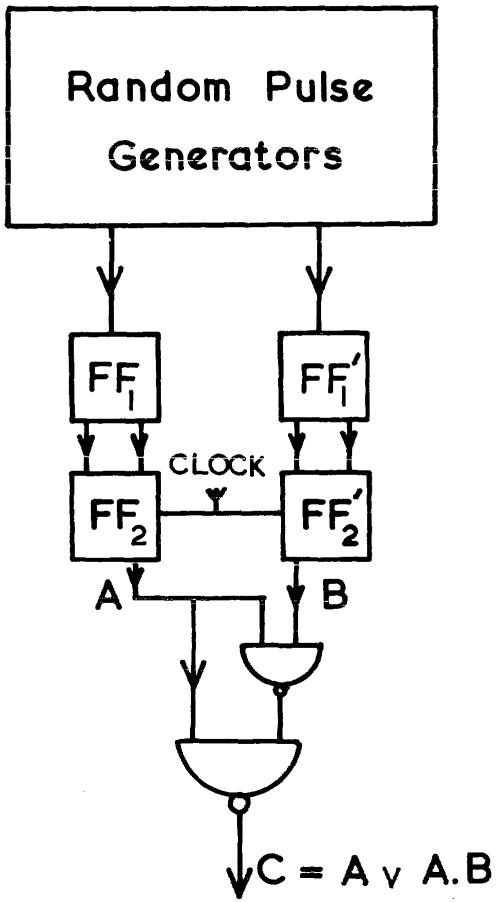
\includegraphics[width=0.6\textwidth, height=7cm, keepaspectratio]{images/86d4c25b150612ffb31e1017b90576a3917bdbf1872594a8388c5304573a1f6b.jpg}
    \caption{随机序列的生成$(p = 3/4)$}
\end{figure}

目前正在建造中的 Mark II 型随机计算机采用了完全不同的技术，既减小了体积和成本，又将时钟频率提高到了1兆周. 采用一个单一的中央伪随机移位寄存器来为所有计算单元生成随机序列. 通过适当的异或门选通移位寄存器输出，可以获得移位寄存器本身序列的延迟副本，从而为每个单元提供不同的序列. 图 11 展示了这样一种生成器，它使用43个触发器，能够在无交叉重复的情况下为一百个16位积分器提供一小时的随机序列.

\begin{figure}[htbp]
    \centering
    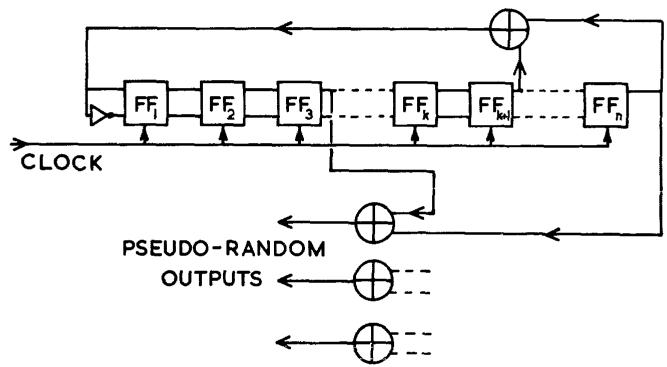
\includegraphics[width=0.6\textwidth, height=7cm, keepaspectratio]{images/e461dd2b34742f61ee15e7f93e5f386678fa36ebbf7e38c1db4fface1c924d3e.jpg}
    \caption{中央伪随机生成器}
\end{figure}

Mark II 型计算机的积分器采用串行运算，因此可以使用移位寄存器实现计数器，并使用少得多的门电路实现比较器. 通过这种方式，现在可以用仅六个双列直插式封装来制造一个十六位随机积分器. 移位寄存器中的16兆周时钟频率在随机计算机中产生1兆周的时钟频率，现在可以实现约100周的相当可观的带宽.
